\documentclass[aspectratio=169,t]{beamer}

% Clean academic look: white background, no decorations
\usetheme{default}
\setbeamertemplate{navigation symbols}{}
\setbeamercolor{background canvas}{bg=white}
\setbeamercolor{normal text}{fg=black}
\setbeamercolor{frametitle}{fg=black}
\setbeamerfont{frametitle}{size=\large, series=\bfseries}
\setbeamertemplate{frametitle}{%
  \vspace{0.6em}\hspace{0.5em}\insertframetitle\par}
\setbeamertemplate{footline}{%
  \hfill\scriptsize\color{gray!70}\insertframenumber\;/\;\inserttotalframenumber\hspace{1em}\vspace{0.4em}}
\setbeamertemplate{itemize item}{\textbullet}
\setbeamertemplate{itemize subitem}{--}

\usepackage{booktabs}
\usepackage{amsmath, amssymb}
\usepackage{xcolor}
\usepackage{graphicx}
\usepackage{tabularx}
\usepackage{array}
\usepackage{tikz}
\usetikzlibrary{matrix, positioning, arrows.meta}

% Compact tables
\renewcommand{\arraystretch}{1.05}

% Path for figures (relative to this .tex's compile dir)
\graphicspath{{./}{../../outputs/figs/}{../../outputs/figs/longitudinal/}{../../outputs/figs/io/}{../../outputs/figs/proc/}}

% Convenience commands
\newcommand{\pia}{\pi_{\alpha}}
\newcommand{\sigxi}{\sigma_{\xi}}
\newcommand{\siga}{\sigma_{\alpha}}
\newcommand{\sigr}{\sigma_{r}}
\newcommand{\sigz}{\sigma_{\zeta}}
\newcommand{\siglam}{\sigma_{\lambda}}
\newcommand{\delt}{\delta}

% Highlight color for newly-added term in each spine build slide.
\definecolor{newterm}{RGB}{195,30,55}
\newcommand{\new}[1]{\textcolor{newterm}{\boldsymbol{#1}}}
\newcommand{\old}[1]{\textcolor{black!45}{#1}}

\title{\bfseries A Bayesian Standard Model of Early Word Learning}
\subtitle{Joint inference across vocabulary, input, and processing data}
\author{Michael C.\ Frank}
\institute{\small Stanford University}
\date{April 2026}

\begin{document}

% =====================================================================
\begin{frame}[plain]
\titlepage
\end{frame}

% =====================================================================
\begin{frame}{Goal: model how language input drives vocabulary learning}

A unified statistical model of early word learning, organized around
four research questions:

\vspace{0.6em}
\begin{description}
\item[\textbf{RQ1.}] How well does word frequency reconstruct word
  difficulty? \par
  \emph{i.e., is $\psi_j \approx -\log p_j$ enough?}
\item[\textbf{RQ2.}] When does word learning start? \par
  \emph{is start time $s$ identifiable from data?}
\item[\textbf{RQ3.}] Does vocabulary growth accelerate over development?\par
  \emph{is $\delta$ greater than 0?}
\item[\textbf{RQ4.}] How much of between-child vocabulary variance is
  driven by input rate vs.\ learning efficiency? \par
  \emph{what is $\pi_\alpha = \siga^2 / (\siga^2 + \sigr^2)$?}
\end{description}

\vspace{0.6em}
\small
\textit{Follow-up to Kachergis, Marchman, \& Frank (2021):
``Toward a standard model of early language learning.''}

\end{frame}

% =====================================================================
\begin{frame}{Motivation: how much variation is there to explain?}

\begin{columns}[T, onlytextwidth]

\column{0.55\textwidth}
Fit the simplest possible 1-PL IRT — \(P(y_{aj}=1) = \sigma(\theta_a - \beta_j)\) — to the longitudinal Wordbank data. No accumulator dynamics, just per-admin \(\theta_a\), per-item \(\beta_j\).

\vspace{0.4em}
\textbf{Population age slope:} 0.47 logits/mo.

\textbf{Within-age SD}\,(\(\theta_a\)): 1.95 logits.

\vspace{0.4em}
\textbf{Translation:}
\[
\underbrace{\frac{\mathrm{SD}_{\mathrm{within-age}}}{\hat\beta_{\mathrm{age}}}}_{\text{months / SD}} \;=\; \frac{1.95}{0.47} \;\approx\; \mathbf{4.2~months}
\]

\textbf{And it grows with age:} 1.0 logit at 12--14\,mo (\(\sim\)2\,mo) \(\to\) 2.7 logits at 26--30\,mo (\(\sim\)5.8\,mo).  Children fan out, not converge.

\column{0.45\textwidth}
\centering
\includegraphics[width=\linewidth]{precursor_trajectories.png}

\vspace{0.6em}
\footnotesize\textit{Per-admin \(\theta_a\) for each of \(\sim\)200 English children.  Median 4 admins/kid.  Black: pop.\ age slope.}
\end{columns}

\vspace{0.6em}
\footnotesize
\textbf{Why this matters for the model.}  A pure accumulator with constant per-child rate cannot produce growing spread.  We need age-varying child-level dynamics.  The remainder of this talk builds and tests a model family that does.

\end{frame}

% =====================================================================
\begin{frame}{Schematic model: bucket-fill metaphor + item-response theory}

\begin{columns}[c, onlytextwidth]
\column{0.55\textwidth}
\textbf{Two ideas from Kachergis et al.\ (2021):}
\begin{enumerate}
\item \emph{Accumulator.}
  Each word is a bucket; child hears tokens at rate $r_i \cdot p_j$;
  efficiency $\alpha_i$ determines fraction retained.
\item \emph{Item-Response Theory.}
  Per-word difficulty $\psi_j$ controls how many ``filled'' tokens
  it takes for the child to know the word.
\end{enumerate}

\column{0.45\textwidth}
\centering
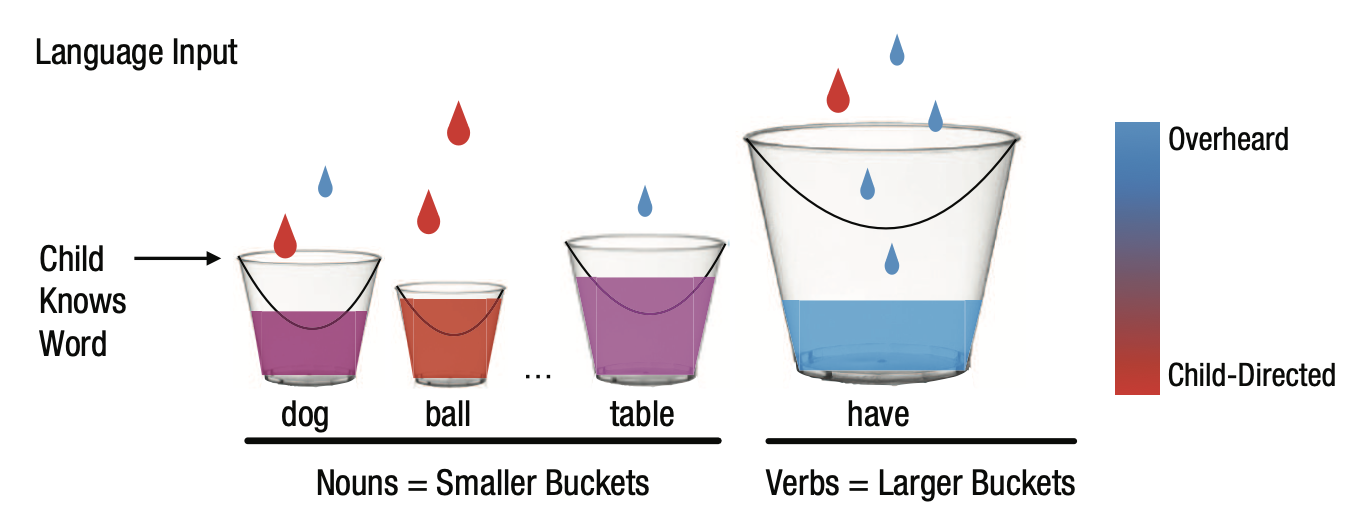
\includegraphics[width=\linewidth]{kachergis_buckets.png}
\end{columns}

\end{frame}

% =====================================================================
\begin{frame}[fragile]{Model: linear predictor (anatomy)}

$P(\text{produces}_{ijt} = 1) = \mathrm{logit}^{-1}(\eta_{ijt})$
where:

\vspace{1.2em}
\centering
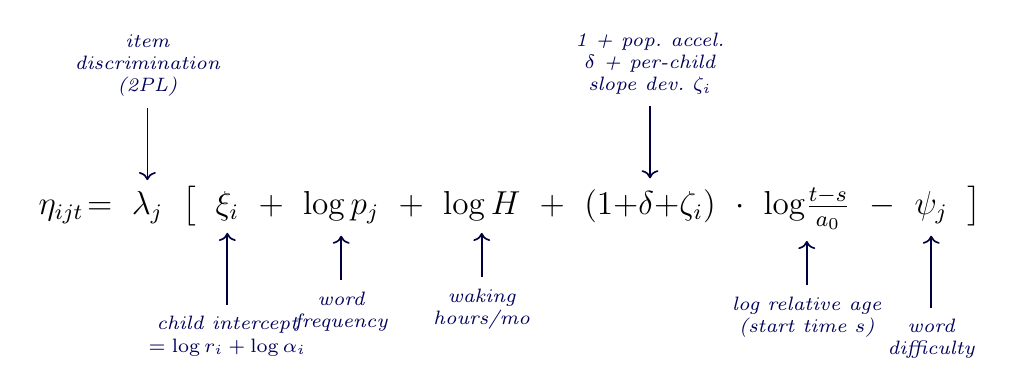
\begin{tikzpicture}[
  every node/.style={inner sep=2pt},
  ann/.style={font=\scriptsize\itshape, color=blue!35!black, align=center},
  arrow/.style={->, blue!25!black, semithick, shorten >=2pt, shorten <=2pt}
]

\matrix[matrix of nodes, column sep=3pt, nodes={font=\large},
        ampersand replacement=\&] (eq) {
  $\eta_{ijt}\!=$ \&
  |[name=lambda]| $\lambda_j$ \&
  $\big[$ \&
  |[name=xi]| $\xi_i$ \&
  $+$ \&
  |[name=logp]| $\log p_j$ \&
  $+$ \&
  |[name=logH]| $\log H$ \&
  $+$ \&
  |[name=slope]| $(1{+}\delta{+}\zeta_i)$ \&
  $\cdot$ \&
  |[name=logage]| $\log\!\tfrac{t-s}{a_0}$ \&
  $-$ \&
  |[name=psi]| $\psi_j$ \&
  $\big]$ \\
};

% Above-equation annotations
\node[ann, above=3.0em of lambda] (a_lambda) {item\\discrimination\\(2PL)};
\draw[arrow] (a_lambda) -- (lambda);

\node[ann, above=3.0em of slope] (a_slope) {1 + pop.\ accel.\\$\delta$ + per-child\\slope dev.\ $\zeta_i$};
\draw[arrow] (a_slope) -- (slope);

% Below-equation annotations
\node[ann, below=3em of xi] (a_xi) {child intercept\\$=\log r_i + \log\alpha_i$};
\draw[arrow] (a_xi) -- (xi);

\node[ann, below=2em of logp] (a_logp) {word\\frequency};
\draw[arrow] (a_logp) -- (logp);

\node[ann, below=2em of logH] (a_logH) {waking\\hours/mo};
\draw[arrow] (a_logH) -- (logH);

\node[ann, below=2em of logage] (a_logage) {log relative age\\(start time $s$)};
\draw[arrow] (a_logage) -- (logage);

\node[ann, below=3em of psi] (a_psi) {word\\difficulty};
\draw[arrow] (a_psi) -- (psi);

\end{tikzpicture}

\end{frame}

% =====================================================================
\begin{frame}[fragile]{Factorization: ability vs.\ difficulty}

The same equation regrouped as a 2PL IRT factorization:
\[
\eta_{ijt} \;=\; \lambda_j \cdot \big(\,\theta_{it} \;-\; \beta_j\,\big)
\]

\vspace{0.4em}
\begin{columns}[T, onlytextwidth]

% ---------- Ability constellation ----------
\column{0.50\textwidth}
\centering
\textbf{Ability} (child $+$ age):\\[0.3em]
$\theta_{it} = \xi_i + (1{+}\delta{+}\zeta_i)\,\log\!\tfrac{t-s}{a_0}$

\vspace{0.8em}
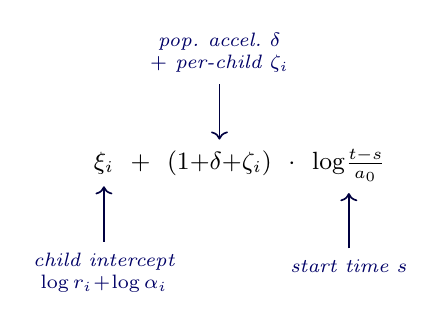
\begin{tikzpicture}[
  every node/.style={inner sep=2pt},
  ann/.style={font=\scriptsize\itshape, color=blue!40!black, align=center},
  arrow/.style={->, blue!25!black, semithick, shorten >=2pt, shorten <=2pt}
]
\matrix[matrix of nodes, column sep=2pt, nodes={font=\small},
        ampersand replacement=\&] (eqA) {
  |[name=Axi]| $\xi_i$ \&
  $+$ \&
  |[name=Aslope]| $(1{+}\delta{+}\zeta_i)$ \&
  $\cdot$ \&
  |[name=Aage]| $\log\!\tfrac{t-s}{a_0}$ \\
};
\node[ann, below=2.4em of Axi]    (aAxi)   {child intercept\\$\log r_i\!+\!\log\alpha_i$};
\draw[arrow] (aAxi) -- (Axi);
\node[ann, above=2.4em of Aslope] (aAslope){pop.\ accel.\ $\delta$\\$+$ per-child $\zeta_i$};
\draw[arrow] (aAslope) -- (Aslope);
\node[ann, below=2.4em of Aage]   (aAage)  {start time $s$};
\draw[arrow] (aAage) -- (Aage);
\end{tikzpicture}

% ---------- Difficulty constellation ----------
\column{0.50\textwidth}
\centering
\textbf{Difficulty} (item):\\[0.3em]
$\beta_j = \psi_j - \log p_j - \log H$

\vspace{0.8em}
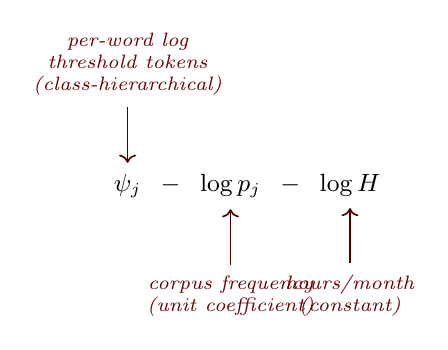
\begin{tikzpicture}[
  every node/.style={inner sep=2pt},
  ann/.style={font=\scriptsize\itshape, color=red!40!black, align=center},
  arrow/.style={->, red!30!black, semithick, shorten >=2pt, shorten <=2pt}
]
\matrix[matrix of nodes, column sep=3pt, nodes={font=\small},
        ampersand replacement=\&] (eqB) {
  |[name=Bpsi]| $\psi_j$ \&
  $-$ \&
  |[name=Blogp]| $\log p_j$ \&
  $-$ \&
  |[name=BlogH]| $\log H$ \\
};
\node[ann, above=2.4em of Bpsi]  (aBpsi)  {per-word log\\threshold tokens\\(class-hierarchical)};
\draw[arrow] (aBpsi) -- (Bpsi);
\node[ann, below=2.4em of Blogp] (aBlogp) {corpus frequency\\(unit coefficient)};
\draw[arrow] (aBlogp) -- (Blogp);
\node[ann, below=2.4em of BlogH] (aBlogH) {hours/month\\(constant)};
\draw[arrow] (aBlogH) -- (BlogH);
\end{tikzpicture}

\end{columns}

\vspace{0.6em}
\footnotesize
\textbf{Why split it.}  $\log p_j$ and $\log H$ together convert
``probability'' into ``expected tokens per month at unit input rate,''
so they pair naturally on the item side.  Each ablation lives on
exactly one side: \textit{pin $\delta=0$, free $s$, drop $\zeta_i$}
touch \textbf{ability}; \textit{drop class hierarchy, class-specific
$\beta_c$} (planned) touch \textbf{difficulty}; \textit{2PL}
($\lambda_j$) is a multiplier on the $(\theta-\beta)$ gap.  LWL
processing speed (Peekbank) informs $\theta$ via $\log\alpha_i$.

\end{frame}

% =====================================================================
\begin{frame}{Model variants}

\textbf{Per-child latents.}
$(\log\alpha_i, \zeta_i) \sim \mathrm{MVN}\!\big(0,\Sigma\big)$
with LKJ prior on the correlation; $\log r_i \sim N(\mu_r, \sigr)$
independent. \emph{Sum-to-zero centering on each random effect}
identifies $\delta$ (population slope) separately from
$\mathrm{mean}(\zeta_i)$.

\vspace{0.6em}
\textbf{Lean baseline + opt-in variants.}
Pin $s\!=\!0$, $\siglam\!=\!0$, $\sigz\!=\!0$ by default; opt in
explicitly:

\vspace{0.4em}
\centering
\small
\begin{tabular}{ll}
\toprule
variant & adds \\
\midrule
\texttt{slopes}     & $\zeta_i$, $\sigz$ \,(longitudinal default) \\
\texttt{2pl}        & $\lambda_j$, $\siglam$ \\
\texttt{free\_s}    & free $s$ \\
\texttt{fix\_delta} & $\delta = 0$ \\
\bottomrule
\end{tabular}

\flushleft
\vspace{0.6em}
\textbf{$\sigr$ pinned externally} from Sperry / Hart-Risley /
Weisleder-Fernald data; lets the model decompose
$\sigxi^2 = \sigr^2 + \siga^2$ and report $\pia$.

\end{frame}

% =====================================================================
\begin{frame}{Main longitudinal sample: Wordbank English + Norwegian}

\textbf{Data.} Wordbank longitudinal CDIs (WG $\cup$ WS forms).
Children with $\ge 2$ admins; both forms count toward the same child.

\vspace{0.6em}
\begin{tabular}{lrrr}
\toprule
 & N children & N admins & age range (mo) \\
\midrule
English (American) & 200 & $\sim$808 & 8--32 \\
Norwegian          & 200 & $\sim$1\,594 & 8--32 \\
\bottomrule
\end{tabular}

\vspace{1em}
\textbf{Stratified subsampling.}
\begin{itemize}
\item \textbf{Children}: 4 age-bins on median admin age, equal $n$ per
  bin; favor those with most admins / longest spans.
\item \textbf{Items}: $4 \times 4$ stratification on (lexical class
  $\times$ $\log p_j$ quartile). 200 items kept.
\end{itemize}

\vspace{0.5em}
\textbf{Stan.} \texttt{log\_irt\_long.stan}; 4 chains $\times$ 1000
iter $\times$ 500 warmup; adapt\_delta = 0.95; runs in 3--8 hours
on Sherlock.

\end{frame}

% =====================================================================
\begin{frame}{Results: lean baseline (English, slopes only)}

\begin{columns}[T, onlytextwidth]
\column{0.45\textwidth}
\textbf{Headline scalars} (post.\ med.\ {[}95\% CrI{]}):
\vspace{0.3em}
\small
\begin{tabular}{lr}
\toprule
\multicolumn{2}{l}{\textbf{Population}} \\
\midrule
$\siga$    & 1.83 \,[1.65,\,2.04] \\
$\sigxi$   & 1.90 \,[1.73,\,2.11] \\
$\sigz$    & 3.48 \,[3.05,\,3.96] \\
$\rho_{\xi\zeta}$ & 0.40 \,[0.27,\,0.53] \\
$\delt$    & 9.39 \,[8.58,\,10.2] \\
$s$        & 0.52 \,(pinned) \\
$\boldsymbol{\pia}$ & \textbf{0.913 \,[0.901,\,0.926]} \\
\bottomrule
\end{tabular}

\vspace{0.4em}
\textit{Efficiency variance dominates input variance: $\pia \approx 0.91$.}

\column{0.55\textwidth}
\centering
\includegraphics[width=\linewidth]{english_ablations_trajectory.png}
\end{columns}

\end{frame}

% =====================================================================
\begin{frame}{Nested family: build the model one component at a time}

We test each component's contribution by building a strictly nested
spine. Every step \emph{adds one named component}, and every step has
a fit on disk so we can compare it to its predecessor by LOO ELPD.

\vspace{0.6em}
\centering
\small
\renewcommand{\arraystretch}{1.15}
\begin{tabular}{@{}clp{0.42\linewidth}p{0.30\linewidth}@{}}
\toprule
\textbf{stage} & \textbf{adds} & \textbf{interpretation} & \textbf{answers} \\
\midrule
M0 & --                       & minimal IRT: per-child $\xi_i$, per-word $\psi_j$, no time, no frequency & identifiability anchor \\
M1 & $+\;\log\!\frac{t-s}{a_0}$         & per-child accumulation grows with log-age (unit slope) & basic accumulator \\
M2 & $+\;\log p_j$            & per-token frequency channel (unit coef) & \textbf{RQ2:} does freq matter? \\
M3 & $+\;\delta$              & population-level age acceleration & \textbf{RQ1:} does growth accelerate? \\
M4 & $+\;\zeta_i$             & per-child slope deviation around $\delta$ & between-child rate variance \\
M5 & $+\;\beta_c\!\cdot\!\log p_j$ & class-specific frequency coefficient & class $\times$ freq interaction \\
M6 & $+\;\lambda_j$           & per-word discrimination (2PL) & item-level sharpness \\
\bottomrule
\end{tabular}

\vspace{0.6em}
\footnotesize
The next 7 slides walk through each stage's linear predictor, with the
newly-added term highlighted. Implementation: each stage corresponds
to a single \texttt{variant\_hyperpriors()} entry that toggles the
relevant prior from "tight near zero" to "free."

\end{frame}

% ====== M0 ===========================================================
\begin{frame}[fragile]{M0: minimal IRT (no time, no frequency)}

\vspace{0.8em}
\centering
\Large
$\eta_{ijt} = \xi_i + \log H - \psi_j$

\vspace{1.6em}
\normalsize
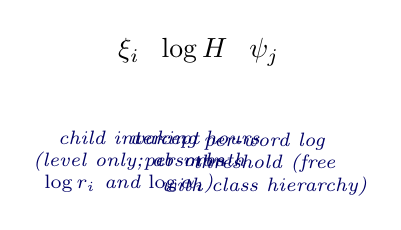
\begin{tikzpicture}[every node/.style={inner sep=2pt},
  ann/.style={font=\scriptsize\itshape, color=blue!40!black, align=center},
  arrow/.style={->, blue!25!black, semithick, shorten >=2pt, shorten <=2pt}]
\matrix[matrix of nodes, column sep=4pt, ampersand replacement=\&]{
  |[name=Mxi]| $\xi_i$ \&
  |[name=MlogH]| $\log H$ \&
  |[name=Mpsi]| $\psi_j$ \\
};
\node[ann, below=2.0em of Mxi]   {child intercept\\(level only; absorbs\\$\log r_i$ and $\log \alpha_i$)};
\node[ann, below=2.0em of MlogH] {waking hours\\per month};
\node[ann, below=2.0em of Mpsi]  {per-word log\\threshold (free\\with class hierarchy)};
\end{tikzpicture}

\vspace{1.4em}
\footnotesize
\textbf{What this is.} The simplest possible item-response model: a
fixed-in-age "ability" per child, a fixed difficulty per word, no
mechanism. Vocabulary curves are flat in age; differences across
children all live in $\xi_i$.

\textbf{Why M0 first.} Establishes the identifiability anchor for
$\xi_i$ (free per child) and $\psi_j$ (free per word with class prior).
Subsequent stages add structural channels on top of these.

\end{frame}

% ====== M1 ===========================================================
\begin{frame}[fragile]{$\boldsymbol{M_1 = M_0\;+\;\text{time}}$}

\vspace{0.8em}
\centering
\Large
$\eta_{ijt} = \old{\xi_i + \log H} + \new{\log\!\tfrac{t-s}{a_0}} - \old{\psi_j}$

\vspace{1.4em}
\normalsize
{\color{newterm}\textbf{Time term:}} the child's accumulation grows
with the log of (age $-$ start time), at a fixed unit slope.

\vspace{1.6em}
\centering
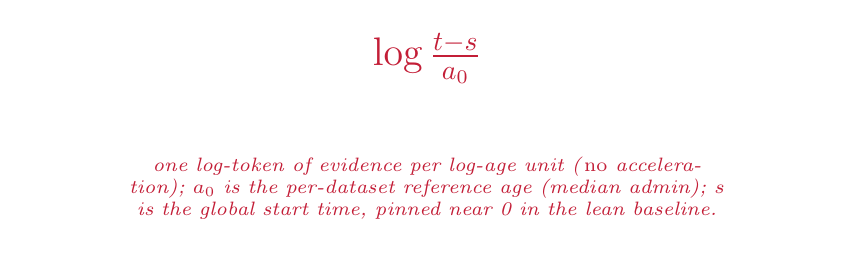
\begin{tikzpicture}[every node/.style={inner sep=2pt},
  ann/.style={font=\scriptsize\itshape, color=newterm, align=center},
  arrow/.style={->, newterm, semithick, shorten >=2pt, shorten <=2pt}]
\node[font=\Large, color=newterm] (T) {$\log\tfrac{t-s}{a_0}$};
\node[ann, below=2.2em of T, text width=10cm]
  {one log-token of evidence per log-age unit (\emph{no} acceleration);
   $a_0$ is the per-dataset reference age (median admin); $s$ is the
   global start time, pinned near 0 in the lean baseline.};
\end{tikzpicture}

\vspace{1.4em}
\footnotesize
\textbf{What's pinned.} $\delta = 0$ (no acceleration), $\beta_c = 0$
(no frequency channel), $\zeta_i = 0$, $\lambda_j = 1$. Equivalent to
McMurray's (2007) deterministic accumulator without the frequency
proxy or any per-child age dynamics beyond a constant log-age slope.

\end{frame}

% ====== M2 ===========================================================
\begin{frame}[fragile]{$\boldsymbol{M_2 = M_1\;+\;\text{frequency}}$}

\vspace{0.8em}
\centering
\Large
$\eta_{ijt} = \old{\xi_i + \log H} + \new{\log p_j} + \old{\log\!\tfrac{t-s}{a_0}} - \old{\psi_j}$

\vspace{1.4em}
\normalsize
{\color{newterm}\textbf{Frequency term:}} per-token corpus frequency
of word $j$ in CHILDES, with unit coefficient ("one log-token of
evidence per log-token of corpus probability").

\vspace{1.6em}
\centering
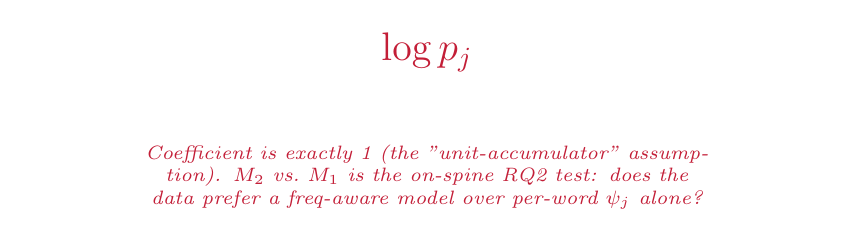
\begin{tikzpicture}[every node/.style={inner sep=2pt},
  ann/.style={font=\scriptsize\itshape, color=newterm, align=center},
  arrow/.style={->, newterm, semithick, shorten >=2pt, shorten <=2pt}]
\node[font=\Large, color=newterm] (P) {$\log p_j$};
\node[ann, below=2.2em of P, text width=10cm]
  {Coefficient is exactly 1 (the "unit-accumulator" assumption).
   $M_2$ vs.\ $M_1$ is the on-spine RQ2 test: does the data prefer
   a freq-aware model over per-word $\psi_j$ alone?};
\end{tikzpicture}

\vspace{1.4em}
\footnotesize
\textbf{What's still pinned.} $\delta = 0$, $\zeta_i = 0$,
$\beta_c = 1$ (unit), $\lambda_j = 1$.

\end{frame}

% ====== M3 ===========================================================
\begin{frame}[fragile]{$\boldsymbol{M_3 = M_2\;+\;\delta\text{ (acceleration)}}$}

\vspace{0.8em}
\centering
\Large
$\eta_{ijt} = \old{\xi_i + \log H + \log p_j} + (1{+}\new{\delta})\old{\log\!\tfrac{t-s}{a_0}} - \old{\psi_j}$

\vspace{1.4em}
\normalsize
{\color{newterm}\textbf{Acceleration:}} the population log-age slope
becomes $1 + \delta$ instead of $1$. With $\delta > 0$, evidence
accumulates super-linearly in log-age $\Leftrightarrow$ token weight
grows with development.

\vspace{1.6em}
\centering
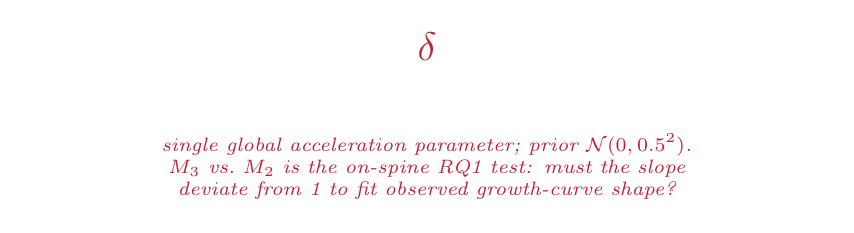
\begin{tikzpicture}[every node/.style={inner sep=2pt},
  ann/.style={font=\scriptsize\itshape, color=newterm, align=center},
  arrow/.style={->, newterm, semithick, shorten >=2pt, shorten <=2pt}]
\node[font=\Large, color=newterm] (D) {$\delta$};
\node[ann, below=2.2em of D, text width=10cm]
  {single global acceleration parameter; prior $\mathcal{N}(0, 0.5^2)$.
   $M_3$ vs.\ $M_2$ is the on-spine RQ1 test: must the slope deviate
   from 1 to fit observed growth-curve shape?};
\end{tikzpicture}

\vspace{1.4em}
\footnotesize
\textbf{What's still pinned.} $\zeta_i = 0$, $\beta_c = 1$, $\lambda_j = 1$.

\end{frame}

% ====== M4 ===========================================================
\begin{frame}[fragile]{$\boldsymbol{M_4 = M_3\;+\;\zeta_i\text{ (per-child slopes)}}$}

\vspace{0.8em}
\centering
\Large
$\eta_{ijt} = \old{\xi_i + \log H + \log p_j} + (1{+}\delta{+}\new{\zeta_i})\old{\log\!\tfrac{t-s}{a_0}} - \old{\psi_j}$

\vspace{1.4em}
\normalsize
{\color{newterm}\textbf{Per-child slope deviation:}} on top of the
population acceleration, each child has their own $\zeta_i$ — a
deviation of the log-age slope around $\delta$.

\vspace{1.6em}
\centering
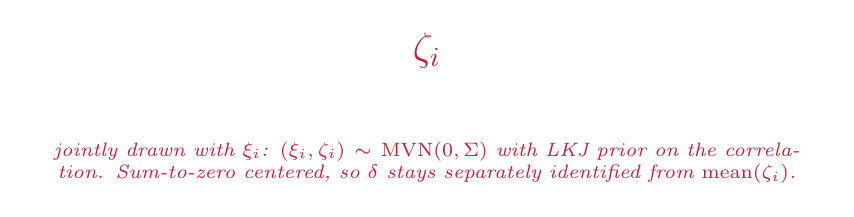
\begin{tikzpicture}[every node/.style={inner sep=2pt},
  ann/.style={font=\scriptsize\itshape, color=newterm, align=center},
  arrow/.style={->, newterm, semithick, shorten >=2pt, shorten <=2pt}]
\node[font=\Large, color=newterm] (Z) {$\zeta_i$};
\node[ann, below=2.2em of Z, text width=10cm]
  {jointly drawn with $\xi_i$:
   $(\xi_i, \zeta_i) \sim \mathrm{MVN}(0, \Sigma)$ with LKJ prior on
   the correlation. Sum-to-zero centered, so $\delta$ stays separately
   identified from $\mathrm{mean}(\zeta_i)$.};
\end{tikzpicture}

\vspace{1.4em}
\footnotesize
\textbf{What's still pinned.} $\beta_c = 1$, $\lambda_j = 1$. Adding
$\zeta_i$ requires \emph{longitudinal} data to identify; the
cross-sectional version of this fit is unidentified.

\end{frame}

% ====== M5 ===========================================================
\begin{frame}[fragile]{$\boldsymbol{M_5 = M_4\;+\;\beta_c\text{ (class-specific freq)}}$}

\vspace{0.8em}
\centering
\Large
$\eta_{ijt} = \old{\xi_i + \log H} + \new{\beta_{c(j)}}\old{\log p_j + (1{+}\delta{+}\zeta_i)\log\!\tfrac{t-s}{a_0} - \psi_j}$

\vspace{1.4em}
\normalsize
{\color{newterm}\textbf{Class-specific frequency coefficient:}} the
unit weight on $\log p_j$ becomes a per-class free parameter $\beta_c$,
one for each lexical class (nouns, predicates, function words, other).

\vspace{1.6em}
\centering
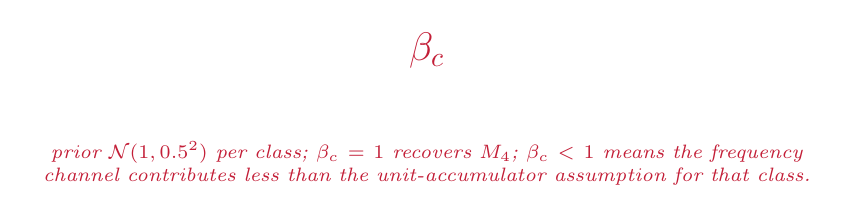
\begin{tikzpicture}[every node/.style={inner sep=2pt},
  ann/.style={font=\scriptsize\itshape, color=newterm, align=center},
  arrow/.style={->, newterm, semithick, shorten >=2pt, shorten <=2pt}]
\node[font=\Large, color=newterm] (B) {$\beta_c$};
\node[ann, below=2.2em of B, text width=10cm]
  {prior $\mathcal{N}(1, 0.5^2)$ per class; $\beta_c = 1$ recovers $M_4$;
   $\beta_c < 1$ means the frequency channel contributes less than the
   unit-accumulator assumption for that class.};
\end{tikzpicture}

\vspace{1.4em}
\footnotesize
\textbf{What's still pinned.} $\lambda_j = 1$.

\end{frame}

% ====== M6 ===========================================================
\begin{frame}[fragile]{$\boldsymbol{M_6 = M_5\;+\;\lambda_j\text{ (2PL discrimination)}}$}

\vspace{0.8em}
\centering
\Large
$\eta_{ijt} = \new{\lambda_j}\,\old{\big[\,\xi_i + \log H + \beta_{c(j)}\log p_j + (1{+}\delta{+}\zeta_i)\log\!\tfrac{t-s}{a_0} - \psi_j\,\big]}$

\vspace{1.4em}
\normalsize
{\color{newterm}\textbf{Per-word discrimination:}} the entire ability
$-$ difficulty gap is multiplied by a word-specific $\lambda_j$. High
$\lambda_j$ = sharp transition near $\psi_j$ (concrete nouns); low
$\lambda_j$ = gradual transition (function words, abstracts).

\vspace{1.6em}
\centering
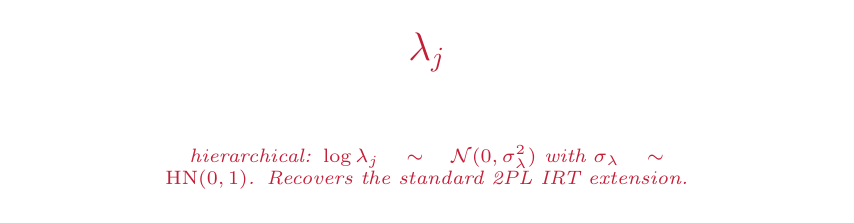
\begin{tikzpicture}[every node/.style={inner sep=2pt},
  ann/.style={font=\scriptsize\itshape, color=newterm, align=center},
  arrow/.style={->, newterm, semithick, shorten >=2pt, shorten <=2pt}]
\node[font=\Large, color=newterm] (L) {$\lambda_j$};
\node[ann, below=2.2em of L, text width=10cm]
  {hierarchical: $\log \lambda_j \sim \mathcal{N}(0, \sigma_\lambda^2)$
   with $\sigma_\lambda \sim \mathrm{HN}(0,1)$. Recovers the standard
   2PL IRT extension.};
\end{tikzpicture}

\vspace{1.4em}
\footnotesize
\textbf{Full model.} $M_6$ has the complete linear predictor as
introduced on slide~5; everything to its left is now structurally
free (or unit-anchored where the data prefer that).

\end{frame}

% ====== LOO results ==================================================
\begin{frame}{Spine LOO comparison (English, $N=200$ children)}

\vspace{0.4em}
\textbf{Step-wise ELPD differences} (later $-$ earlier, $\sigma_r=0.534$ pinned):

\vspace{0.4em}
\centering
\small
\renewcommand{\arraystretch}{1.18}
\begin{tabular}{@{}lrrrl@{}}
\toprule
step & $\Delta$ELPD & SE & $z$ & verdict \\
\midrule
$M_1\;\text{vs}\;M_0$ & $+8\,033$  & 36   & 222.6 & \textbf{time matters} \\
$M_2\;\text{vs}\;M_1$ & $\sim\!0$ (pending) & -- & -- & \textbf{RQ2:} on-spine; new fit running \\
$\boldsymbol{M_3\;\text{vs}\;M_2}$ & $\boldsymbol{+23\,289}$ & $\boldsymbol{178}$ & $\boldsymbol{131.0}$ & \textbf{RQ1: $\delta$ matters, decisively} \\
$M_4\;\text{vs}\;M_3$ & $+2\,212$  & 69   & 31.9  & per-child slopes matter \\
$M_5\;\text{vs}\;M_4$ & $+1.5$     & 1.25 & 1.2   & class $\beta_c$ \emph{null} \\
$M_6\;\text{vs}\;M_5$ & $+1\,079$  & 52   & 20.8  & 2PL marginal but real \\
\bottomrule
\end{tabular}

\vspace{0.8em}
\flushleft
\footnotesize
\textbf{Reading the table.}
\begin{itemize}\setlength\itemsep{0.15em}
\item RQ1 (acceleration): closed at $z = 131$. The $\delta$ step is the
  load-bearing structural addition.
\item RQ2 (frequency): the off-spine M4-level test gave
  $z = 0.5$ (drop $\log p_j$, no ELPD change). On-spine $M_2\!\!\to\!\!M_1$
  test pending Sherlock job 23710155.
\item M5 (class-specific $\beta_c$): null at the LOO level
  ($z = 1.2$). The per-class posteriors $(0.55, 0.45, 0.36, 0.16)$
  trade off cleanly with $\psi_j$; no out-of-sample value.
\item Best by LOO: $M_6$. Recommended adopt-and-augment scaffold:
  $M_4$ (slopes-level), with the no-frequency variant as M\_best for
  input-uptake fits.
\end{itemize}

\end{frame}

% =====================================================================
\begin{frame}{Why we want input-uptake datasets}

The longitudinal fit \textbf{infers} $\sigr$ from external Sperry-style
priors. To \emph{measure} between-child input variance directly, we
need datasets with per-child observed input rates.

\vspace{0.6em}
\begin{tabularx}{\linewidth}{lXX}
\toprule
& \textbf{BabyView} (Long et al.\ 2025) &
\textbf{SEEDLingS} (Bergelson; Egan-Dailey 2025) \\
\midrule
Recording channel & head-mounted body camera + transcript & passive
LENA all-day audio \\
Observer effect   & \textbf{yes} ($\beta_{\mathrm{react}}$ free) &
\textbf{no} ($\beta_{\mathrm{react}}$ pinned at 0) \\
N kids (post-link) & 20 & 44 \\
CDI form          & WG $\cup$ WS, longitudinal & WG, 6--18\,mo \\
Per-recording rate & $\log r^{\mathrm{obs}}_v$ from FEM/MAL tokens &
$\log r^{\mathrm{obs}}_v$ from LENA AWC \\
\bottomrule
\end{tabularx}

\vspace{0.4em}
\textbf{Modeling.} Same Stan model (\texttt{log\_irt\_io.stan});
$\beta_{\mathrm{react}}$ on/off via dataset-level prior.

\end{frame}

% =====================================================================
\begin{frame}{IO results: $\pia$ replicates across samples}

\begin{columns}[T, onlytextwidth]
\column{0.5\textwidth}
\centering
\small\textbf{BabyView io\_slopes} (N=20)
\includegraphics[width=\linewidth]{babyview_io_input.png}

\column{0.5\textwidth}
\centering
\small\textbf{SEEDLingS io\_slopes} (N=44)
\includegraphics[width=\linewidth]{seedlings_io_input.png}
\end{columns}

\vspace{0.2em}
\centering
\footnotesize
\begin{tabular}{lrrrr}
\toprule
dataset & N kids & $\pia$ & $\delt$ & $\siga$ \\
\midrule
English (long\_slopes)        & 200 & 0.91 [0.90, 0.93] & 9.39 & 1.83 \\
BabyView (io\_slopes)         &  20 & 0.86 [0.73, 0.94] & 6.40 & 1.20 \\
SEEDLingS (io\_slopes)        &  44 & \textbf{0.99 [0.99, 1.00]} & 8.04 & 2.59 \\
\bottomrule
\end{tabular}

\vspace{0.1em}
\scriptsize\textit{Three samples, two input-observation methods,
one unobserved-input baseline: efficiency variance dominates.}

\end{frame}

% =====================================================================
\begin{frame}{Peekbank experiment: LWL as a window onto $\log\alpha$}

\textbf{Sample.} 62 Adams \& Marchman (2018) children with both LWL
RT/accuracy from Peekbank (247 admins, 13--20\,mo) and item-level
CDIs at 22 + 25\,mo from the Stanford TotLot 3 cohort.

\vspace{0.6em}
\textbf{Joint model.}
\[
\log \mathrm{rt}_{i,t} \sim \mathcal{N}\!\big(
\mu_{rt} + \mu_{\mathrm{rtslope}}\,\ell_t
\;-\; \boldsymbol{\gamma_{rt}}\,\log \alpha_i
\;+\; \ell_t\,\mathrm{rtslope}_i,
\;\sigma_{\mathrm{lwl}}\big)
\]
where $\ell_t = \log(t/a_0)$.
$(\log \alpha, \zeta, \mathrm{rtslope}) \sim \mathrm{MVN}$
with LKJ prior on the correlation matrix.

\vspace{0.6em}
\textbf{Result.}
\begin{itemize}\setlength\itemsep{0.2em}
\item $\boldsymbol{\gamma_{rt} = 0.073}$ \,[0.032,\,0.117]
  -- bounded away from zero. Each unit of $\log \alpha$ corresponds
  to \textasciitilde{}12\% lower mean RT.
\item $\mu_{\mathrm{rtslope}} = -0.73$: RT \emph{decreases} with age,
  expected.
\item $\sigma_{\mathrm{rtslope}} = 0.74$: real per-child variation in
  RT-improvement rate.
\end{itemize}

\end{frame}

% =====================================================================
\begin{frame}{Comparison to prior accumulator models}

\centering
\scriptsize
\renewcommand{\arraystretch}{1.15}
\begin{tabular}{@{}lccccc@{}}
\toprule
Model & Per-child & Per-word & Acceleration & Bayesian & Real units \\
\midrule
McMurray 2007                 & --                          & $g(\tau)$               & via $g'$                & --              & --     \\
Mitchell \& McMurray 2009     & --                          & $g(\tau)$ + leverage    & via $g'$                & --              & --     \\
Hidaka 2013                   & --                          & $(N, \delta, D)$        & via $D$                 & --              & --     \\
Mollica \& Piantadosi 2017    & --                          & $(k_w, \lambda_w)$      & --                      & $\checkmark$    & partial \\
Kachergis et al.\ 2021        & $\theta_i$                  & $d_j$, class            & --                      & --              & --     \\
\textbf{Ours (M5)}            & $\xi_i, \zeta_i, \pia$      & $\psi_j, \lambda_j, \beta_c$ & $\delta$ free        & $\checkmark$    & $\checkmark$ \\
\bottomrule
\end{tabular}

\vspace{1.2em}
\footnotesize
\textbf{What's new in our nested family.}
\begin{itemize}\setlength\itemsep{0.15em}
\item McMurray 2007 / Mitchell \& McMurray 2009: deterministic, no per-child variation.  Their $g'(\tau) > 0$ requirement maps onto our \textbf{M2 vs.\ M1} test (does $\delta > 0$?).
\item Hidaka 2013: closed-form Gamma / Weibull AoA distributions, population-averaged. Our \textbf{M1, M2, M3} occupy the same family (cumulative, rate-change, both) at the per-(child, word, age) Bernoulli level.
\item Mollica \& Piantadosi 2017: $(k_w, \lambda_w)$ Gamma waiting time; large-$k$ approximated by our logistic. Their joint $(k, \lambda)$ ridge is our $(s, \delta)$ ridge.
\item Kachergis et al.\ 2021: standardized logit IRT.  Our model adds external $\sigma_r$ pin (RQ3), structural $\delta$ (RQ1), real token units, and observation-channel architecture (uptake / processing).
\end{itemize}

\flushleft
\scriptsize\textit{Full mathematical mapping in the explainer §\,Comparison to prior accumulator models.}

\end{frame}

% =====================================================================
\begin{frame}{Conclusions}

\begin{itemize}\setlength\itemsep{0.6em}
\item $\pia \approx 0.86$--$0.99$ \emph{across three samples}:
  between-child vocabulary variance is driven primarily by efficiency,
  not input rate.
\item $\delta \approx 6$--$9$ \emph{across all variants}: vocabulary
  growth genuinely accelerates with age; pinning $\delta = 0$ breaks
  population fit.
\item LWL processing speed informs $\log\alpha$ in the expected
  direction; coupling $\gamma_{rt} > 0$ is bounded away from zero.
\end{itemize}

\vspace{1em}
\small\textit{Code, data, fits, and full explainer:
\texttt{github.com/langcog/standard-model-2}}

\end{frame}

\end{document}
